\documentclass[12pt]{report}

\usepackage{graphicx}
\graphicspath{ {image/} }
\usepackage[a4paper,width=165mm,top=25mm,bottom=25mm]{geometry}
\usepackage{caption}

\title{
    {\textbf{Predicting Strength of High-Performance Concrete Using Artificial Neural Network}}\\
}
\author{$by$\\
	\textbf{Mayank Pathania}\\
	\textbf{Roll No. - 204103314}\\
	\vspace{1in}
	\textbf{Specialization - Machine Design}\\
	{
\includegraphics[scale=0.2]{images/university.png}}\\
	{\large \textbf{Indian Institute of Technology, Guwahati}}\\
	{\large \textbf{Guwahati - 781039, India}}
}

\date{\textbf{\today}}

\begin{document}
\maketitle
\tableofcontents

\setcounter{chapter}{1} 
\setcounter{section}{0}
\setcounter{figure}{0}
\setcounter{table}{0}
\chapter*{Introduction}
\addcontentsline{toc}{chapter}{1. Introduction}
\section{Problem Definition}
Concrete is the most important material in civil engineering. The concrete compressive strength is a highly nonlinear function of age and ingredients.\\
The objective of the problem is to predict the strength of High-performance concrete based on some parameters.
There are mainly 8 parameters Cement, Blast Furnace Slag, Fly Ash, Water, Super-plasticizer, Coarse Aggregate, Fine Aggregate and Age that effect the strength of the High-performance concrete. The mathematical modeling of such system is not easy and is highly non-linear. So a soft computing technique, Artificial Neural Network, is used to test if it is possible to predict the Strength using Artificial Neural Network and given parameters.

\section{Attribute Information}
The data is taken from UCI Machine Learning Repository.\\
In table 1.1 the name for the component, type of data, Measurement units and description whether input or output variable is given. The order of the components is in table same as ordered in the data files.\\
\begin{center}
\begin{tabular}{|c|c|c|c|}
\hline
Name & Data Type & Measurement & Description\\
\hline
Cement & quantitative & kg in a m3 mixture & Input Variable\\
\hline
Blast Furnace Slag & quantitative & kg in a m3 mixture & Input Variable\\
\hline
Fly Ash & quantitative & kg in a m3 mixture & Input Variable\\
\hline
Water & quantitative & kg in a m3 mixture & Input Variable\\
\hline
Superplasticizer & quantitative & kg in a m3 mixture & Input Variable\\
\hline
Coarse Aggregate & quantitative & kg in a m3 mixture & Input Variable\\
\hline
Fine Aggregate & quantitative & kg in a m3 mixture & Input Variable\\
\hline
Age & quantitative & Day (1$-$365) & Input Variable\\
\hline
Concrete compressive strength & quantitative & MPa & Output Variable\\
\hline
\end{tabular}
\captionof{table}{Information of components of data}
\end{center}


\setcounter{chapter}{2}
\setcounter{section}{0}
\setcounter{figure}{0}
\setcounter{table}{0}
\chapter*{Methodology}
\addcontentsline{toc}{chapter}{2. Methodology}
\section{Analysing Data}
\hbox{Scatter plots of all the input parameters are plotted with the output parameter(Strength).}
\begin{center}
    \begin{tabular}{cc}
        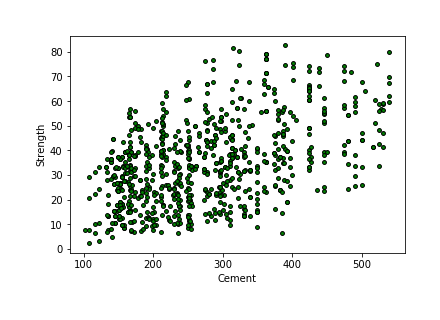
\includegraphics[scale=0.5]{images/Plot_01.png}&
        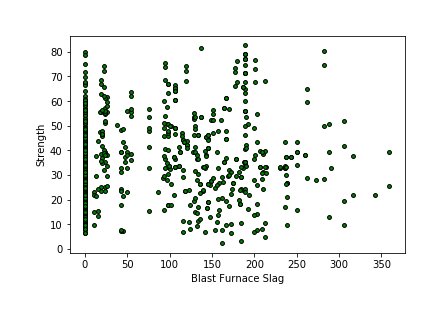
\includegraphics[scale=0.5]{images/Plot_02.png}\\
        a) & b)\\
        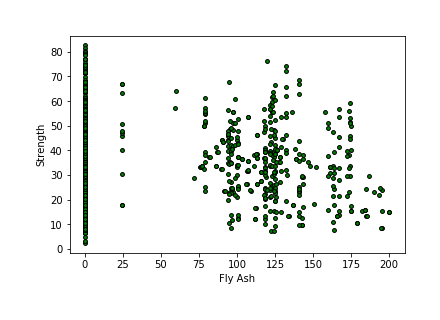
\includegraphics[scale=0.5]{images/Plot_03.png}&
        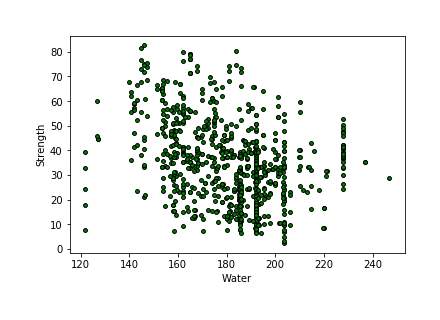
\includegraphics[scale=0.5]{images/Plot_04.png}\\
        c) & d)\\
    \end{tabular}
    \captionof{figure}{Scatter the plots between Strength and a) cement; b) Blast Furnace Slag; c) Fly Ash; d) Water;}
\end{center}
It can be noted that the data is real valued except for Age which is integer valued and it is hard to visualize any linear relationship between input parameters and strength. As it is already mentioned that the relation between strength and input parameters is highly non-linear the a graphs are as expected.\\
For the Cement it can be seen that with the increase of value of cement there is increase in strength but it can also be noted that the strength is highly affected by other parameters as even for high cement values, around $500kgm^{-3}$, strength value varies low to high, around $40MPa$ to $80MPa$.
\begin{center}
    \begin{tabular}{cc}
        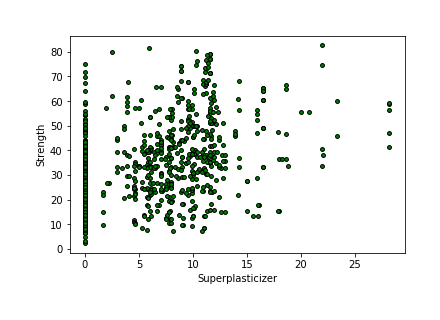
\includegraphics[scale=0.5]{images/Plot_05.png}&
        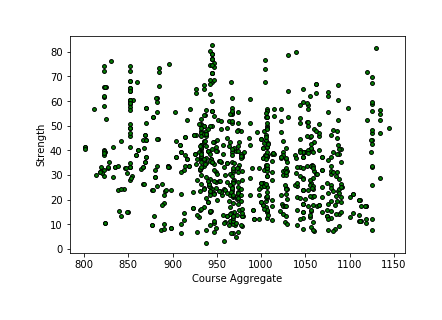
\includegraphics[scale=0.5]{images/Plot_06.png}\\
        a) & b)\\
        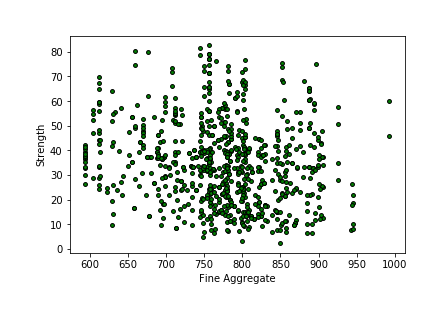
\includegraphics[scale=0.5]{images/Plot_07.png}&
        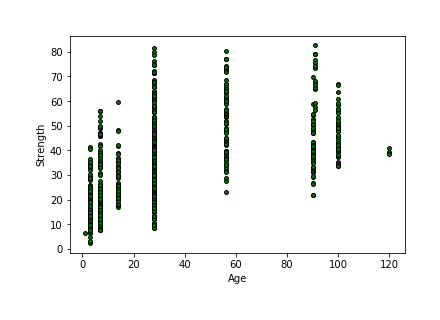
\includegraphics[scale=0.5]{images/Plot_08.png}\\
        c) & d)\\
    \end{tabular}
    \captionof{figure}{Scatter plots between strength and a) Superplasticizer; b) Coarse Aggregate; c) Fine Aggregate; d) Age}
\end{center}

Now the values of data are presented in table to see the maximum, minimum, mean and median of the data in their respective units as discussed in Table 1.1. This tells us the need of normalization of the data as values are not varying in same range and this can lead to baises in prediction. For example cement is ranging form 102 to 540 $kgm^{-3}$ and superplasticizer is ranging from 0 to 22.1 $kgm^{-3}$ this may lead to biases toward cement values.
\begin{center}
    \begin{tabular}{|c|c|c|c|c|}
    	\hline
        $attribute$ & $minimum$ & $maximum$ & $Average$ & $median$\\
        \hline
        $Cement$ & 102.0 & 540.0 & 277.093 & 257.75\\
        \hline
        $Blast Furnace Slag$ & 0.0 & 342.1 & 76.9958 & 22.0\\
        \hline
        $Fly Ash$ & 0.0 & 195.0 & 57.6307 & 0.0\\
        \hline
        $Water$ & 127.0 & 228.0 & 180.1824 & 183.0\\
        \hline
        $Superplasticizer$ & 0.0 & 22.1 & 6.4395 & 7.0\\
        \hline
        $Coarse Aggregate$ & 801.0 & 1145.0 & 976.1921 & 972.2\\
        \hline
        $Fine Aggregate$ & 594.0 & 945.0 & 774.1864 & 778.25\\
        \hline
        $Age$ & 1.0 & 120.0 & 32.3507 & 28.0\\
        \hline
        $Strength$ & 2.33 & 79.4 & 35.415 & 33.724\\
        \hline
    \end{tabular}
	\captionof{table}{Aspect of components of data}
\end{center}

\section{Model Architecture}
The Artificial Neural Network model with one input layer, one hidden layer, and one output layer was considered for the analysis. Model is fully connected network with batch mode of training. The number of input and ouput neurons is 8 and 1 respectively and decided by the number of input and ouput parameters. Number of hidden neurons can be varied.\\
\begin{figure}[h]
	\begin{center}
		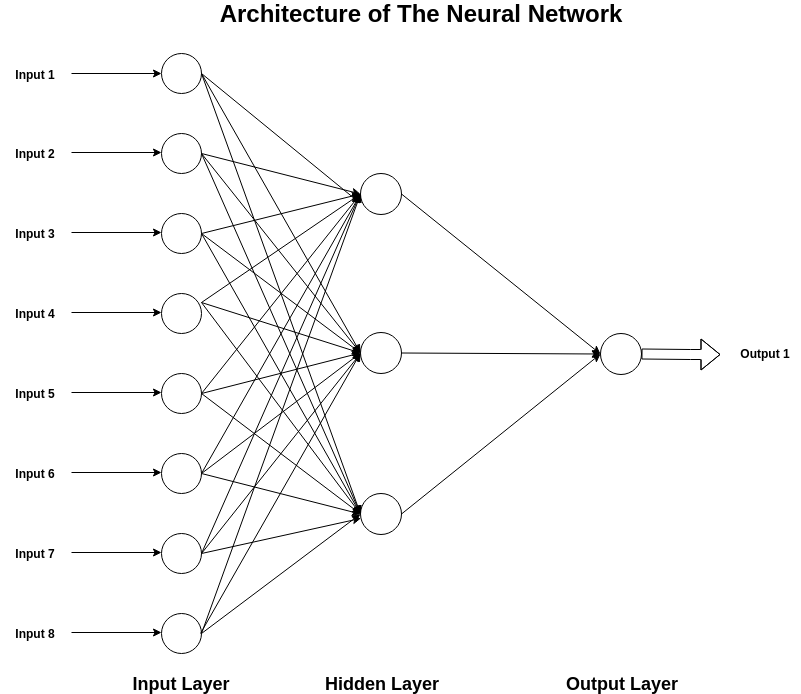
\includegraphics[scale=0.5]{images/architecture.png}
		\captionof{figure}{Architecture of neural network}
	\end{center}
\end{figure}
As the ouput parameter is Strength which is real valued transfer function for both hidden and ouput layer was selected as log sigmoid transfer funciton with a = 1. The values of input parameters were normalized within range -4 to 4 for all parameters before feeding into the network. Also the target values are normalized in the range 0.1 to 0.9.
\begin{center}
		{\huge $y = \frac{1}{1 + e^{-ax}}$}
		\captionof{figure}{Log sigmoid transfer function}
\end{center}


\section{Model Parameters}
Number of hidden neurons, learining rate, momentum coefficient and tolerance value are the model parameters which can be changed to alter the convergence rate and termination criterion of the training. These values were chosen by trial and error method.\\
Different sets of data was feed into the neural network with different model parameters and then number of interations were noted for a given torelance value. Model parameters which gave the best results i.e. minimum number of iterations were chosen as final parameters.\\
\begin{center}
	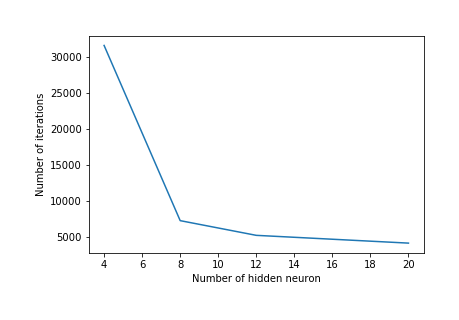
\includegraphics[scale=0.8]{images/iterations/Plot_01.png}
	\captionof{figure}{Comparison of number of iterations for tolerance = $10^{-5}$, learning rate = 0.3 and momentum coefficient = 0}
\end{center}
First the value of learning rate and momentum coefficients were fixed and for hidden neurons 4, 8, 12 and 20 the training was performed and the number of interation taken for training were noted.\\
\begin{center}
	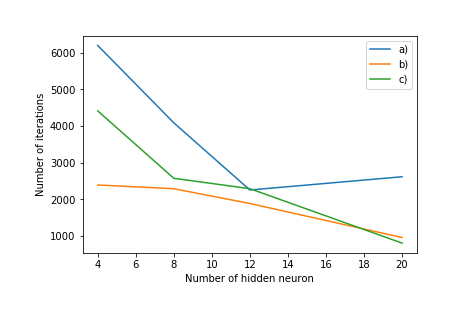
\includegraphics[scale=0.8]{images/iterations/Plot_02.png}
	\captionof{figure}{Comparison of number of iterations for tolerance = $10^{-5}$ and\\ a)learning rate = 0.3 and momentum coefficient = 0\\
		b)learning rate = 0.7 and momentum coefficient = 0.5\\
		c)learning rate = 0.9 and momentum coefficient = 0.6}
\end{center}
Then the values for learning rate and momentum was increased and for different number of hidden neurons again the number of iterations were noted. This process was repeated for various values of model parameters. For this procedure the value of tolerance was taken as $10^{-5}$ but after the selection of parameters the value of tolerance was further decreased to $5\times10^{-6}$ as this increased the accuracy in prediction and increase in number of iterations was not much. But further reduction in tolerance value increased the number of iteration very much.\\
\begin{center}
	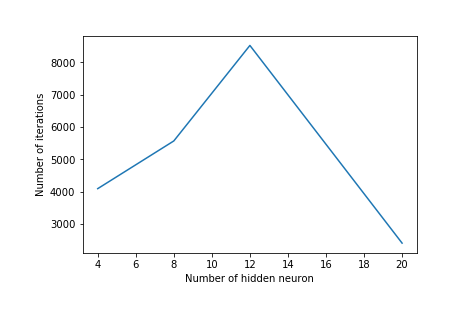
\includegraphics[scale=0.8]{images/iterations/Plot_03.png}
	\captionof{figure}{Comparison of number of iterations for tolerance = $5\times10^{-6}$, learning rate = 0.9 and momentum coefficient = 0.6}
\end{center}
For tolerance, it was noted that for tolerance value of $10^{-6}$ the results of training and testing were good and by further reduction in its value increased the number of iteration but there was not much improvement in predictions. For instance, with tolerance = $10^{-7}$ it took 10 to 20 times more iterations to converge than with tolerance value of $10^{-6}$, but the Mean Square Error for testing in both the cases was of order $10^{-6}$.
\begin{center}
	\begin{tabular}{|c|c|}
		\hline
		\textbf{Model Parameter} & \textbf{Value} \\
		\hline
		No. of Hidden Neurons & 20\\
		\hline
		Learining Rate & 0.9\\
		\hline
		Momentum Coefficients & 0.6\\
		\hline
		Error/Tolerance & $5\times10^{-6}$\\
		\hline
	\end{tabular}
	\captionof{table}{Decided Values of Parameters}
\end{center}

\setcounter{chapter}{3}
\setcounter{section}{0}
\setcounter{figure}{0}
\setcounter{table}{0}
\chapter*{Results and Discussions}
\addcontentsline{toc}{chapter}{3. Results and Discussions}
\section{Convergence Plots}
\begin{center}
	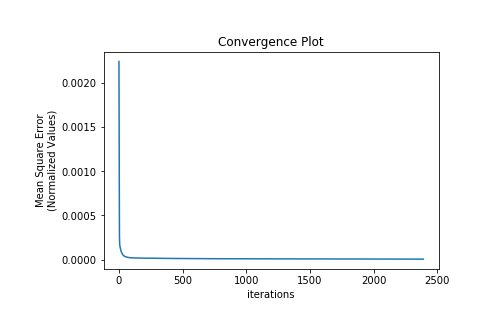
\includegraphics{images/Convergence/Convergence_Plot.png}
	\captionof{figure}{Convergence plot}
\end{center}
The convergence plot is for the selected parameters i.e. No. of hidden neurons = 20, Learning Rate = 0.9, Momentum Coefficients = 0.6 and error/Tolerance = $5\times10^{-6}$. From the convergence plot is can be seen that for the first few iterations, around 5-10, there is major drop in the Mean Square Error(MSE) and after that the curve seems to be flat. To better visualize how the error is reducing after these iterations two more convergence plots are shown in figure 3.2 and figure 3.3.\\
\begin{center}
	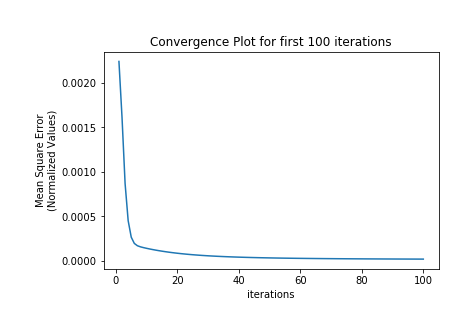
\includegraphics[scale=0.8]{images/Convergence/Convergence_Plot1.png}
	\captionof{figure}{Convergence Plot for first 100 iterations}
\end{center}
From figure 3.2 it can be seen that the reduction in error is very high in first few iterations and around 20 iterations it seems as if the curve is flattening. As the weight values at the start are random the error is high and as the training is proceding the error is reducing.
\begin{center}
	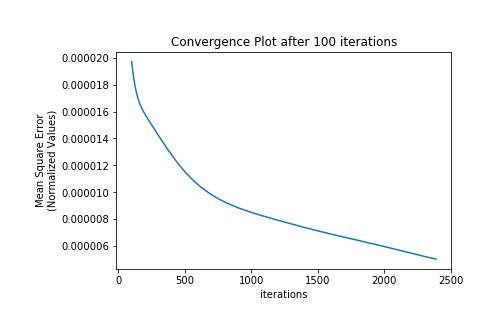
\includegraphics[scale=0.8]{images/Convergence/Convergence_Plot2.png}
	\captionof{figure}{Convergence Plot after 100 iterations}
\end{center}
From figure 3.3 we can appreciate how the error is reducing continuously and the curve actually do not go flat. Even at termination condition curve is quite steep and with further reduction in tolerance value of termination the MSE will further reduce.

\section{Predictions}
\begin{center}
	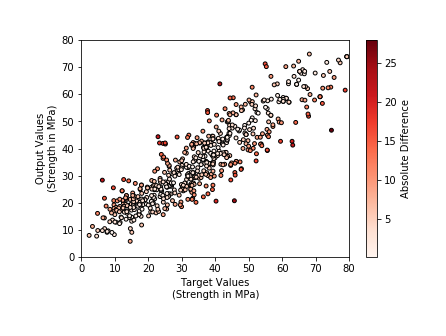
\includegraphics{images/comparison.png}
	\captionof{figure}{Comparison of Target values and Output Values}
\end{center}
Plot in figure 3.4 shows that the prediction values are close to the target values. Variation of Absolute difference between predicted and target values is same throughout. So it cannot be concluded if the method is better for low strength or high strength high-performance concrete. Also the model is Underpredicting and overpredicting by same amount as it can be see by the color which is similar on both sides of portion of the graph with white points.
\begin{center}
	\begin{tabular}{|c|c|}
		\hline
		Maximum absolute Error & 27.9126\\
		\hline
		Minimum absolute Error & 0.0155\\
		\hline
		Mean absolute Error & 5.7182\\
		\hline
		Mean square Error & 52.9724\\
		\hline
	\end{tabular}
	\captionof{table}{Errors in Training Ouput}
\end{center}
\begin{center}
	\begin{tabular}{|c|c|}
		\hline
		Maximum absolute Error & 22.3789\\
		\hline
		Minimum absolute Error & 0.01622\\
		\hline
		Mean absolute Error & 5.3483\\
		\hline
		Mean square Error & 48.7034\\
		\hline
	\end{tabular}
	\captionof{table}{Errors in Testing Ouput}
\end{center}
Tables 3.1 and 3.2 shows various errors in prediction by the ANN Model for training and testing respectively. For both cases the values of errors are almost similar indicating the model has not over-fitted the training data. The maximum absolute error in both cases is high.

\section{Comparison}
In this section a comparison is made between the Model with selected parameters and a model with same parameters and lower tolerance i.e. $10^{-6}$. Though the reduction is only of $5\times10^{-6}$ it will lead to some intersing results.
\subsection{Convergence Plots}
Similar to the section 3.1 here 3 convergece plots are shown in figure 3.5.
\begin{center}
	\begin{tabular}{c}
		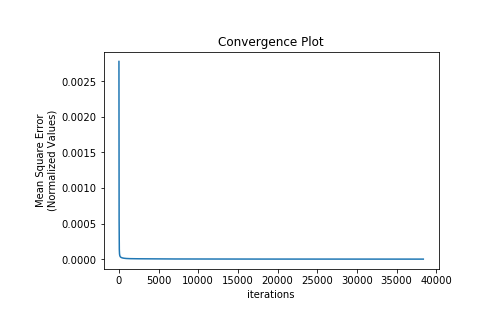
\includegraphics[scale=0.65]{images/comparison/Convergence_Plot_a.png}\\
		a)\\
	\end{tabular}
	\begin{tabular}{cc}
		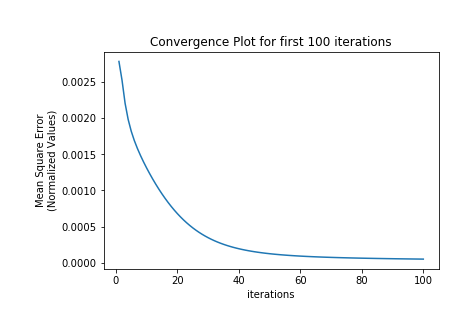
\includegraphics[scale=0.5]{images/comparison/Convergence_Plot1_a.png} & 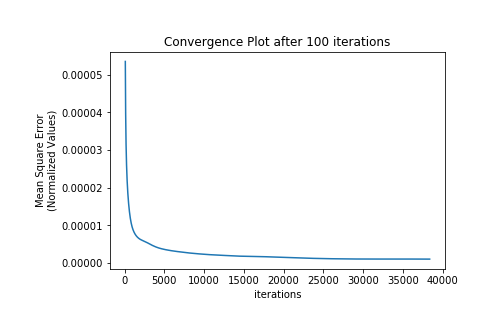
\includegraphics[scale=0.5]{images/comparison/Convergence_Plot2_a.png}\\
		b) & c)\\
	\end{tabular}
	\captionof{figure}{Convergence Plot for a) All iteration; b) First 100 iterations; c) After 100 iterations}
\end{center}
In figure 3.4 a) similar trend can seen in the plot that were seen in figure 3.1. The convergence rate is high in the starting and then it is low as the error is reduced to around $4\times10^{-5}$.\\
From figure 3.5 b) for first 100 iteraton trend is also same that the curve is flattening as the number of iterations are increasing. After 100 iterartions the trend in starting of figure 3.5 c) is similar to figure 3.3 but there is a change in the later stage. At 5000 iterations the error is $3\times10^{-6}$ and after that there is not much change in error and convergence rate is very low and it takes total of 38373 iterations for termination criterion to be fulfiled i.e. $MSE<10^{-6}$. The curve is almost flat in this case while for that in figure 3.3 the curve was quite steep.

\subsection{Predictions}
\begin{center}
	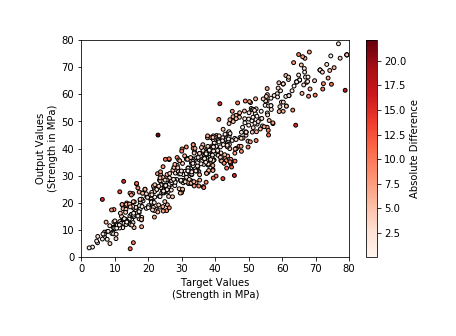
\includegraphics[scale=0.8]{images/comparison/comparison_a.png}
	\captionof{figure}{Comparison of Target values and Output Values}
\end{center}
Plot in figure 3.6 shows that the prediction values are close to the target values. Points are more close to $y=x$ line than in figure 3.4 and also the colors are not as dark for the values.
This implies that most of the predictions are close to the targets and there are lesser number of values which are far from target. This can also be seen from the tables 3.3 and 3.4 that there is a reduction in Mean Square Error and Mean Absolute Error.
\begin{center}
	\begin{tabular}{|c|c|}
		\hline
		Maximum absolute Error & 22.11\\
		\hline
		Minimum absolute Error & 0.005\\
		\hline
		Mean absolute Error & 3.7328\\
		\hline
		Mean square Error & 23.69096\\
		\hline
	\end{tabular}
	\captionof{table}{Errors in Training Ouput}
\end{center}
\begin{center}
	\begin{tabular}{|c|c|}
		\hline
		Maximum absolute Error & 24.924\\
		\hline
		Minimum absolute Error & 0.0625\\
		\hline
		Mean absolute Error & 4.3087\\
		\hline
		Mean square Error & 32.4043\\
		\hline
	\end{tabular}
	\captionof{table}{Errors in Testing Ouput}
\end{center}

\setcounter{chapter}{4}
\setcounter{section}{0}
\setcounter{figure}{0}
\setcounter{table}{0}
\chapter*{Conclusion}
\addcontentsline{toc}{chapter}{4. Conclusion}
High-performance concrete is highly complex matrial and its strength depends on various parameters. 8 parameters were considered and different model parameters for the ANN Model were used to analyse which will give better results and if it is possible to use this technique to predict high-performance concrete.\\
Following Conclusions can be drawn from the study:
\begin{itemize}
	\item This Method can be used to predict the strength of high-performance concrete also ANN model is simple to implement but it will require data and computation resources to train the model upto required accuracy.
	\item Changing the parameters gave different convergence rates. Learning rate = 0.9 was used which is high value but it reduced the number of iterations significantly and did not produced any instability.
	\item Reducing the tolerance value too much might not be helpful as MSE for training will decrease but this might be due to overfitting and during the testing MSE might be only of order $10^{-6}$. More data for training may be helpful but this will also increase the computational time/resources.
\end{itemize}

\section{Some Remarks Regarding Code}
\begin{itemize}
	\item Code is generalized. Input and output parameters can be changes from the file "input\_parameters.dat".
	\item Model parameters can be changed by changing values in the file "model\_parameters.dat". There is only single hidden layer and cannot be changed but number of hidden neurons can be changed.
	\item After training the model for reuse of model "save\_model\_data()" function can be used to save the data and "load\_model\_data()" function can be used to load the saved data.
\end{itemize}

\section*{References}
\addcontentsline{toc}{chapter}{References}
\begin{enumerate}
	\item I-Cheng Yeh, "Modeling of strength of high performance concrete using artificial neural networks," Cement and Concrete Research, Vol. 28, No. 12, pp. 1797-1808 (1998).
\end{enumerate}

\end{document}
